% Options for packages loaded elsewhere
% Options for packages loaded elsewhere
\PassOptionsToPackage{unicode}{hyperref}
\PassOptionsToPackage{hyphens}{url}
\PassOptionsToPackage{dvipsnames,svgnames,x11names}{xcolor}
%
\documentclass[
  letterpaper,
  DIV=11,
  numbers=noendperiod]{scrartcl}
\usepackage{xcolor}
\usepackage{amsmath,amssymb}
\setcounter{secnumdepth}{5}
\usepackage{iftex}
\ifPDFTeX
  \usepackage[T1]{fontenc}
  \usepackage[utf8]{inputenc}
  \usepackage{textcomp} % provide euro and other symbols
\else % if luatex or xetex
  \usepackage{unicode-math} % this also loads fontspec
  \defaultfontfeatures{Scale=MatchLowercase}
  \defaultfontfeatures[\rmfamily]{Ligatures=TeX,Scale=1}
\fi
\usepackage{lmodern}
\ifPDFTeX\else
  % xetex/luatex font selection
\fi
% Use upquote if available, for straight quotes in verbatim environments
\IfFileExists{upquote.sty}{\usepackage{upquote}}{}
\IfFileExists{microtype.sty}{% use microtype if available
  \usepackage[]{microtype}
  \UseMicrotypeSet[protrusion]{basicmath} % disable protrusion for tt fonts
}{}
\makeatletter
\@ifundefined{KOMAClassName}{% if non-KOMA class
  \IfFileExists{parskip.sty}{%
    \usepackage{parskip}
  }{% else
    \setlength{\parindent}{0pt}
    \setlength{\parskip}{6pt plus 2pt minus 1pt}}
}{% if KOMA class
  \KOMAoptions{parskip=half}}
\makeatother
% Make \paragraph and \subparagraph free-standing
\makeatletter
\ifx\paragraph\undefined\else
  \let\oldparagraph\paragraph
  \renewcommand{\paragraph}{
    \@ifstar
      \xxxParagraphStar
      \xxxParagraphNoStar
  }
  \newcommand{\xxxParagraphStar}[1]{\oldparagraph*{#1}\mbox{}}
  \newcommand{\xxxParagraphNoStar}[1]{\oldparagraph{#1}\mbox{}}
\fi
\ifx\subparagraph\undefined\else
  \let\oldsubparagraph\subparagraph
  \renewcommand{\subparagraph}{
    \@ifstar
      \xxxSubParagraphStar
      \xxxSubParagraphNoStar
  }
  \newcommand{\xxxSubParagraphStar}[1]{\oldsubparagraph*{#1}\mbox{}}
  \newcommand{\xxxSubParagraphNoStar}[1]{\oldsubparagraph{#1}\mbox{}}
\fi
\makeatother


\usepackage{longtable,booktabs,array}
\usepackage{calc} % for calculating minipage widths
% Correct order of tables after \paragraph or \subparagraph
\usepackage{etoolbox}
\makeatletter
\patchcmd\longtable{\par}{\if@noskipsec\mbox{}\fi\par}{}{}
\makeatother
% Allow footnotes in longtable head/foot
\IfFileExists{footnotehyper.sty}{\usepackage{footnotehyper}}{\usepackage{footnote}}
\makesavenoteenv{longtable}
\usepackage{graphicx}
\makeatletter
\newsavebox\pandoc@box
\newcommand*\pandocbounded[1]{% scales image to fit in text height/width
  \sbox\pandoc@box{#1}%
  \Gscale@div\@tempa{\textheight}{\dimexpr\ht\pandoc@box+\dp\pandoc@box\relax}%
  \Gscale@div\@tempb{\linewidth}{\wd\pandoc@box}%
  \ifdim\@tempb\p@<\@tempa\p@\let\@tempa\@tempb\fi% select the smaller of both
  \ifdim\@tempa\p@<\p@\scalebox{\@tempa}{\usebox\pandoc@box}%
  \else\usebox{\pandoc@box}%
  \fi%
}
% Set default figure placement to htbp
\def\fps@figure{htbp}
\makeatother


% definitions for citeproc citations
\NewDocumentCommand\citeproctext{}{}
\NewDocumentCommand\citeproc{mm}{%
  \begingroup\def\citeproctext{#2}\cite{#1}\endgroup}
\makeatletter
 % allow citations to break across lines
 \let\@cite@ofmt\@firstofone
 % avoid brackets around text for \cite:
 \def\@biblabel#1{}
 \def\@cite#1#2{{#1\if@tempswa , #2\fi}}
\makeatother
\newlength{\cslhangindent}
\setlength{\cslhangindent}{1.5em}
\newlength{\csllabelwidth}
\setlength{\csllabelwidth}{3em}
\newenvironment{CSLReferences}[2] % #1 hanging-indent, #2 entry-spacing
 {\begin{list}{}{%
  \setlength{\itemindent}{0pt}
  \setlength{\leftmargin}{0pt}
  \setlength{\parsep}{0pt}
  % turn on hanging indent if param 1 is 1
  \ifodd #1
   \setlength{\leftmargin}{\cslhangindent}
   \setlength{\itemindent}{-1\cslhangindent}
  \fi
  % set entry spacing
  \setlength{\itemsep}{#2\baselineskip}}}
 {\end{list}}
\usepackage{calc}
\newcommand{\CSLBlock}[1]{\hfill\break\parbox[t]{\linewidth}{\strut\ignorespaces#1\strut}}
\newcommand{\CSLLeftMargin}[1]{\parbox[t]{\csllabelwidth}{\strut#1\strut}}
\newcommand{\CSLRightInline}[1]{\parbox[t]{\linewidth - \csllabelwidth}{\strut#1\strut}}
\newcommand{\CSLIndent}[1]{\hspace{\cslhangindent}#1}



\setlength{\emergencystretch}{3em} % prevent overfull lines

\providecommand{\tightlist}{%
  \setlength{\itemsep}{0pt}\setlength{\parskip}{0pt}}



 


\usepackage{setspace}
\doublespacing
\usepackage[left]{lineno}
\linenumbers
\usepackage[margin=1in]{geometry}
\KOMAoption{captions}{tableheading}
\makeatletter
\@ifpackageloaded{caption}{}{\usepackage{caption}}
\AtBeginDocument{%
\ifdefined\contentsname
  \renewcommand*\contentsname{Table of contents}
\else
  \newcommand\contentsname{Table of contents}
\fi
\ifdefined\listfigurename
  \renewcommand*\listfigurename{List of Figures}
\else
  \newcommand\listfigurename{List of Figures}
\fi
\ifdefined\listtablename
  \renewcommand*\listtablename{List of Tables}
\else
  \newcommand\listtablename{List of Tables}
\fi
\ifdefined\figurename
  \renewcommand*\figurename{Figure}
\else
  \newcommand\figurename{Figure}
\fi
\ifdefined\tablename
  \renewcommand*\tablename{Table}
\else
  \newcommand\tablename{Table}
\fi
}
\@ifpackageloaded{float}{}{\usepackage{float}}
\floatstyle{ruled}
\@ifundefined{c@chapter}{\newfloat{codelisting}{h}{lop}}{\newfloat{codelisting}{h}{lop}[chapter]}
\floatname{codelisting}{Listing}
\newcommand*\listoflistings{\listof{codelisting}{List of Listings}}
\makeatother
\makeatletter
\makeatother
\makeatletter
\@ifpackageloaded{caption}{}{\usepackage{caption}}
\@ifpackageloaded{subcaption}{}{\usepackage{subcaption}}
\makeatother
\usepackage{bookmark}
\IfFileExists{xurl.sty}{\usepackage{xurl}}{} % add URL line breaks if available
\urlstyle{same}
\hypersetup{
  pdftitle={Literature Review: Selection, QTL Mapping and Statistical Models},
  pdfauthor={Shiyan Miao\textbar u8027892},
  colorlinks=true,
  linkcolor={blue},
  filecolor={Maroon},
  citecolor={Blue},
  urlcolor={Blue},
  pdfcreator={LaTeX via pandoc}}


\title{Literature Review: Selection, QTL Mapping and Statistical Models}
\author{Shiyan Miao\textbar u8027892}
\date{2025-09-08}
\begin{document}
\maketitle

\renewcommand*\contentsname{Table of contents}
{
\hypersetup{linkcolor=}
\setcounter{tocdepth}{3}
\tableofcontents
}

\section{Introduction}\label{introduction}

Selective breeding has been an important tool for agriculture for a long
time. It helped to develop crop varieties and livestock breeds with
higher productivity, better resilience, and improved quality to meet the
global demand for food (Falconer \& Mackay, 1996; Godfray et al., 2010).
However, traditional methods such as phenotypic selection, progeny
testing, and backcrossing are slow and require many resources. They
depend on observable traits, which are often influenced by the
environment, and therefore provide only an indirect and delayed measure
of genetic potential (Collard et al., 2005). So we introduce
marker-assisted analysis to detect traits more efficiently and
accurately.

In genetics, selection means choosing individuals with desirable traits
as parents to produce the next generation, so that favourable alleles
are passed on. Falconer and Mackay (Falconer \& Mackay, 1996) defined
selection as the unequal reproduction of genotypes, caused either by
environmental pressures, which we call natural selection, or by human
choices, which we call artificial selection. Natural selection depends
on environmental effects on survival and reproduction, while artificial
selection depends on human intervention to improve traits of
agricultural or economic importance.

In plant and animal breeding, artificial selection is implemented
through traditional methods such as phenotypic selection, progeny
testing, and backcross breeding. There are three main traditional
breeding methods.\\
\textbf{Phenotypic selection} chooses individuals based on observable
traits or performance, but its accuracy is reduced because environmental
effects can hide genetic differences (Collard et al., 2005).\\
\textbf{Progeny testing} uses the performance of offspring to evaluate
the genetic value of parents; while more reliable, it is expensive and
time-consuming (Foster, 2006).\\
\textbf{Backcross breeding} introduces a favourable allele from a donor
into an elite background through repeated backcrossing, but it requires
many generations and can transfer unwanted linked alleles as well (Wu et
al., 2007).

Therefore, traditional methods such as phenotypic selection, progeny
testing, and backcross breeding have supported crop and livestock
improvement but remain limited by environmental noise, high costs, and
the need for many generations (Collard et al., 2005; Foster, 2006; Wu et
al., 2007). These inefficiencies emphasise the need for more precise and
efficient approaches, leading to the development of marker-assisted
selection (MAS), which uses molecular markers to accelerate and improve
breeding accuracy.

Marker-assisted selection (MAS) is a newer strategy that helps overcome
the limits of these traditional methods. MAS uses DNA markers that are
closely linked to genes of interest to guide breeding decisions,
allowing selection at early growth stages and independent of
environmental variation (Collard et al., 2005; Hasan et al., 2021).
Collard et al. (Collard et al., 2005) showed that MAS is especially
effective for traits with low heritability or late expression. It is
more precise, reliable, and cost-effective than traditional methods.
Hasan et al. (Hasan et al., 2021) also showed that MAS can be used to
combine multiple favourable alleles, making it a powerful tool for crop
and livestock improvement. However, the success of MAS depends on first
identifying markers that are tightly linked to quantitative trait loci
(QTL), which are genomic regions associated with variation in complex
traits (Mackay et al., 2009).

Detecting QTL makes it possible to connect molecular markers with
important phenotypes, but this requires careful statistical analysis.
The following Methods section will provide a more detailed discussion of
how QTL are defined and how statistical models are used to detect them.

In this report, Section 2 reviews statistical methods for detecting QTL,
highlighting their strengths and limitations, while Section 3 presents
discussion and conclusion.

\section{Method}\label{method}

This section introduces the statistical models that are commonly used to
detect quantitative trait loci (QTL). We begin with the single marker
model, which tests the effect of one marker at a time, and then turn to
the multiple marker model, which incorporates several markers
simultaneously to increase power. Multiple marker models, however, often
face challenges such as collinearity, where markers are strongly
correlated, and high dimensionality, where the number of markers is much
larger than the number of samples. To address these issues, we also
review model selection strategies, including stepwise procedures,
Bayesian shrinkage, and penalised regression methods.

\textbf{Statistical method for detecting QTL}

QTL analysis uses data that combine marker genotypes with phenotypic
measurements. Genotypes are often coded numerically (for example, 0 =
homozygous for one allele and 1 = homozygous for the other allele),
which makes it possible to apply statistical models directly (Mackay et
al., 2009). Because the whole genome sequencing is very expensive, QTL
are usually identified indirectly through linkage disequilibrium between
observed markers and unobserved causal loci (Collard et al., 2005).

A quantitative trait locus (QTL) is formally defined as a chromosomal
region containing one or more loci that contribute to variation in a
quantitative trait (Mackay et al., 2009). QTL are not necessarily single
genes; they are often larger genomic regions that contain multiple genes
influencing complex traits such as yield or disease resistance (Collard
et al., 2005). Since QTL cannot be observed directly, their effects must
be inferred statistically by testing associations between marker
genotypes and phenotypic outcomes in a mapping population. Statistical
models provide the framework for this inference by decomposing the
phenotype into genetic and environmental components and by quantifying
how strongly marker genotypes predict trait values (Falconer \& Mackay,
1996).

At their core, these models specify the relationship between a
phenotypic response variable and explanatory variables that represent
marker genotypes. A general form of the model is:

\[
y_i = \beta_0 + \beta_G G_i + \beta_E z_i + \beta_{GE}(G_i \times z_i) + \epsilon_i,
\]

where\\
- \(y_i\) is the phenotype of the \(i\)-th individual (for example,
plant height or yield),\\
- \(\beta_0\) is the intercept, representing the overall mean of the
phenotype,\\
- \(G_i\) is the genetic effect, and \(\beta_G\) is the regression
coefficient for the genetic effect,\\
- \(z_i\) is the environmental effect, and \(\beta_E\) is the regression
coefficient for the environmental effect,\\
- \(G_i \times z_i\) is the interaction between genotype and
environment, and \(\beta_{GE}\) is the coefficient for this
interaction,\\
- \(\epsilon_i\) is the residual error term, which captures random
variation not explained by the model.

For the purposes of this study, the model is simplified to focus only on
the genetic contribution to phenotypic variation:

\[
y_i = \beta_0 + \beta_G G_i + \epsilon_i.
\]

This simplification assumes that environmental effects and
genotype--environment interactions are negligible. As a result, the
analysis considers only the phenotypic variance explained by genetic
effects, while the residual term still accounts for unexplained
variation.

\subsection{Single Marker Model}\label{single-marker-model}

In this study, we focus on a backcross (BC) population, which is
generated by crossing an F1 hybrid back to one of its parental lines. In
the illustrated scheme, an individual homozygous for allele A (blue,
with a star marker) is crossed with an individual homozygous for allele
C (orange, with a star marker). The F1 generation inherits one allele
from each parent and is then crossed again with the recurrent parent
carrying allele C. The backcross design is introduced here because the
single-marker model is formulated using the segregation pattern of this
experimental population.

\begin{figure}

\centering{

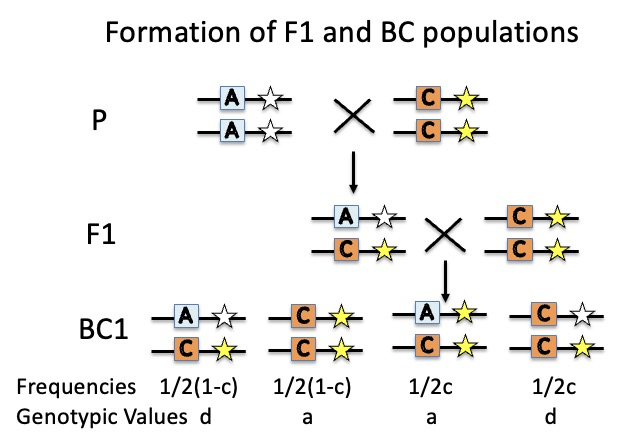
\includegraphics[width=0.7\linewidth,height=\textheight,keepaspectratio]{Figure 4.jpg}

}

\caption{\label{fig-1}}

\end{figure}%

As shown in the figure, recombination between the marker locus and the
putative QTL occurs with probability \(c\), the recombination fraction.
The resulting BC₁ progeny segregate into four possible genotypes:

With probability \(\tfrac{1}{2}(1-c)\), the offspring inherit the
non-recombinant haplotype associated with genotypic value \(d\).

With probability \(\tfrac{1}{2}(1-c)\), they inherit the alternate
non-recombinant haplotype with genotypic value \(a\).

With probability \(\tfrac{1}{2}c\), recombination produces a haplotype
with genotypic value \(a\).

With probability \(\tfrac{1}{2}c\), recombination produces a haplotype
with genotypic value \(d\).

\subsubsection{Mean Difference between
Genotypes}\label{mean-difference-between-genotypes}

In QTL analysis, the relationship between a marker and a QTL can be
described using the recombination frequency (\(c\)), which measures how
often crossover occurs between loci. The recombination fraction (\(c\))
not only shows how strong the linkage is between two loci, but it can
also be used to build a genetic map. By turning the recombination rate
between markers into genetic distance measured in centimorgans (cM), and
using LOD scores to test if the linkage is significant, researchers can
place markers in order along the chromosome (Collard et al., 2005). When
\(c=0\), the loci are completely linked; when \(c=0.5\), they segregate
independently (Falconer \& Mackay, 1996). In practice, markers that are
tightly linked to a QTL act as useful proxies because recombination is
rare (Mackay et al., 2009). Based on these recombination probabilities,
we can calculate the expected phenotypic mean for each genotype. For
example, the expected values for AC and CC genotypes can be expressed
as:

\[
\mu_{AC} = \tfrac{1}{2}(1-c)d + \tfrac{1}{2}ca, \qquad
\mu_{CC} = \tfrac{1}{2}(1-c)a + \tfrac{1}{2}cd
\]

Since QTL detection is concerned with whether genotypes differ in their
average phenotypes, we focus on the difference between these means. We
define this difference as

\[
\Delta = \mu_{AC} - \mu_{CC},
\]

where \(\Delta\) represents the expected phenotypic difference between
the two genotypes. Substituting the above expressions gives:

\[
\Delta = (d-a)(1-2c).
\]

This shows that when \((d-a)=0\), there is no genetic effect, and when
\(c=0.5\), the marker and QTL are unlinked (Yang, 2019). The difference
\(\Delta\) can also be written in a regression framework.

\subsubsection{Univariate Regression}\label{univariate-regression}

The difference \(\Delta\) is essentially the average effect of the
marker on the phenotype. In statistical terms, this corresponds to the
regression coefficient \(\beta\) in a simple linear regression model.
Thus, the regression framework provides a formal way to test the same
biological relationship.

In a BC population with only two genotypes (AC and CC), the single
marker regression model is:

\[
y_i = \mu + \beta G_i + \epsilon_i,
\]

where \(G_i\) is coded as 0 for AC and 1 for CC, and \(\beta\) is equal
to the difference \(\Delta\). This formulation allows us to test whether
\(\beta\) differs significantly from zero using a t-test (Foster, 2006),
providing a straightforward way to evaluate marker--QTL association.

It shows how recombination frequency and genetic effects can be
translated into a simple linear model that links marker genotype with
phenotype.

\subsubsection{Mixture Distribution}\label{mixture-distribution}

While the regression model summarises genotype differences using mean
values, it assumes normally distributed residuals within each genotype.
In practice, phenotypic distributions may be more complex. To capture
this, mixture models extend the analysis by modelling the full
distribution of phenotypes conditional on marker genotypes.

In a BC1 population, we assume there is a single QTL linked to the
marker with recombination fraction \(c\). Because the BC design involves
crossing an F1 heterozygote (Qq) with a homozygous recessive parent
(qq), the possible QTL genotypes among the progeny are Qq and qq. Under
this assumption, the conditional probabilities of QTL genotype given the
observed marker genotype are:

\begin{itemize}
\tightlist
\item
  If the marker genotype is AC:
\end{itemize}

\[
P(Qq \mid AC) = 1-c, \qquad P(qq \mid AC) = c
\]

\begin{itemize}
\tightlist
\item
  If the marker genotype is CC:
\end{itemize}

\[
P(Qq \mid CC) = c, \qquad P(qq \mid CC) = 1-c
\] (Foster, 2006, p. 15).

\begin{figure}

\centering{

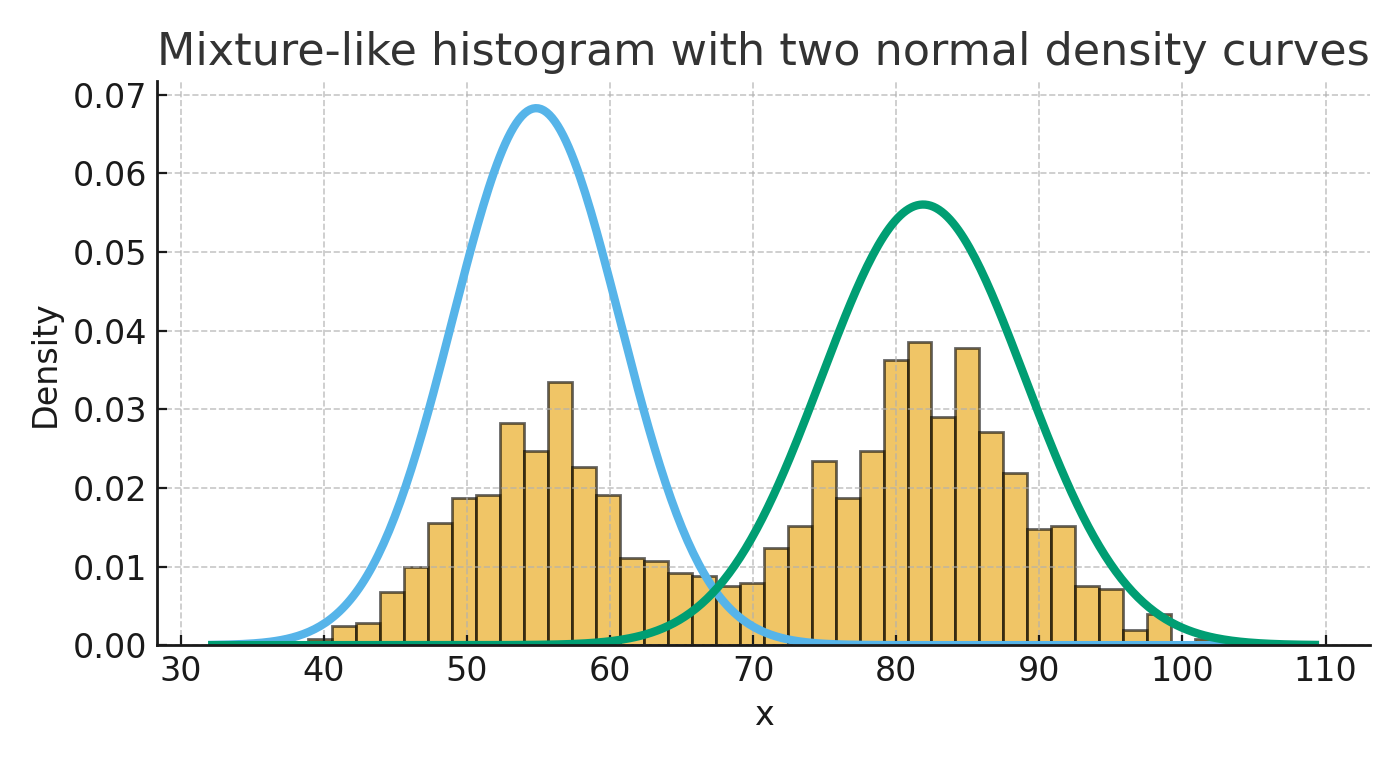
\includegraphics[width=0.7\linewidth,height=\textheight,keepaspectratio]{Figure 2.png}

}

\caption{\label{fig-2}}

\end{figure}%

The phenotype density conditional on marker genotype is defined as:

\[
f(z \mid AC) = (1-c)\,\varphi\!\left(z;\mu_{Qq},\sigma^2\right) + c\,\varphi\!\left(z;\mu_{qq},\sigma^2\right)
\]

\[
f(z \mid CC) = c\,\varphi\!\left(z;\mu_{Qq},\sigma^2\right) + (1-c)\,\varphi\!\left(z;\mu_{qq},\sigma^2\right).
\]

Here, \(z\) denotes the observed phenotype of an individual (e.g., plant
height or yield). \(\mu_{Qq}\) and \(\mu_{qq}\) are the expected
phenotypic means for QTL genotypes Qq and qq, respectively. \(\sigma^2\)
is the residual variance, which captures variation not explained by
genotype, such as environmental effects or measurement error. The
function \(\varphi(z \mid \mu,\sigma^2)\) is the normal density:

\[
\varphi(z \mid \mu,\sigma^2) \;=\; \frac{1}{\sqrt{2\pi\sigma^2}}\,
\exp\!\left(-\frac{(z-\mu)^2}{2\sigma^2}\right).
\]

The overall phenotypic distribution is therefore a two-component normal
mixture (Foster, 2006; Wu et al., 2007).

The single marker model provides a simple and intuitive framework for
QTL detection. By comparing the phenotypic means of different marker
classes in a backcross population, we can express their difference as
\(\Delta = (d-a)(1-2c)\) and reformulate this difference as the
regression coefficient \(\beta\) in a univariate regression. This model
is powerful for illustrating the basic relationship between markers and
QTL, and it can be tested statistically using a t-test. However, its
main limitation is that it considers one locus at a time and does not
control for the effects of other loci. As a result, spurious
associations may occur and true QTL effects may be underestimated.

\subsection{Multiple Marker Model}\label{multiple-marker-model}

In contrast to single-marker analysis, which tests one locus at a time,
the multiple marker model simultaneously incorporates information from
several markers across the genome into a linear regression framework.
This approach improves statistical power by accounting for background
loci and reduces spurious associations that may arise when only one
marker is analysed in isolation.

Formally, the model can be expressed as:

\[
y_i = \mu + \sum_{j=1}^{m} \beta_j G_{ij} + \epsilon_i,
\]

where

\begin{itemize}
\tightlist
\item
  \(y_i\) is the phenotypic value of the \(i\)-th individual,\\
\item
  \(G_{ij}\) denotes the coded genotype of the \(j\)-th marker for the
  \(i\)-th individual (for example, 0/1 coding for backcross
  populations; 0/1/2 coding for F\(_2\) populations),\\
\item
  \(\beta_j\) represents the partial regression coefficient, capturing
  the effect of marker \(j\) conditional on the presence of other
  markers in the model,\\
\item
  \(\mu\) is the overall mean, and\\
\item
  \(\epsilon_i \sim \mathcal{N}(0, \sigma^2)\) denotes the residual
  error term, assumed to follow an independent and identically
  distributed normal distribution.
\end{itemize}

In multiple marker models, traditional methods include stepwise
regression and model choice based on information criteria such as the
Akaike Information Criterion (AIC) and the Bayesian Information
Criterion (BIC). In recent years, penalised regression methods have
become more common. Ridge regression uses an \(\ell_2\) penalty to
shrink coefficients and produce more stable results when markers are
highly correlated (Ogutu et al., 2012). The LASSO method applies an
\(\ell_1\) penalty, which both selects important variables and controls
their size (Li \& Sillanpää, 2012). The elastic net combines \(\ell_1\)
and \(\ell_2\) penalties. This gives a balance between variable
selection and stability, and works well in high-dimensional data where
markers show strong correlation (Brault et al., 2021; Zou \& Hastie,
2005).

we will introduce each of these methods in details for the rest of the
section.

\subsubsection{Stepwise Selection}\label{stepwise-selection}

A classical approach to variable selection is stepwise regression, in
which markers are iteratively added or removed from the model according
to predefined criteria. In practice, the AIC and BIC are widely used to
select the model that minimises information loss:

\[
\text{AIC} = -2 \log L + 2k, \qquad 
\text{BIC} = -2 \log L + k \log n,
\]

where \(L\) is the likelihood of the model, which is a measure of how
well the model fits the data, \(k\) the number of parameters, and \(n\)
the sample size.

Stepwise procedures are computationally straightforward and
interpretable. However, they are known to be unstable in
high-dimensional genomic contexts and fail to account for model
uncertainty, often leading to overconfident inference (Foster, 2006).

\subsubsection{Bayesian Shrinkage}\label{bayesian-shrinkage}

A more flexible alternative is Bayesian shrinkage, in which regression
coefficients are assigned hierarchical priors that adaptively control
the degree of shrinkage for each marker. For marker effect \(\beta_j\),
a zero-mean normal prior is assumed:

\[
\beta_j \sim \mathcal{N}\!\left(0, \frac{\sigma^2}{\lambda_j}\right),
\]

where \(\lambda_j\) is a marker-specific precision parameter. To
complete the hierarchy, a Gamma prior is placed on \(\lambda_j\):

\[
\lambda_j \sim \text{Gamma}(a,b).
\]

where \(a\) and \(b\) are hyperparameters that control the shape of the
Gamma prior.

In the normal--gamma prior, the size of \(\lambda_j\) controls the
amount of shrinkage. A larger \(\lambda_j\) produces stronger shrinkage,
which pulls \(\beta_j\) closer to zero, while a smaller \(\lambda_j\)
allows \(\beta_j\) to take larger values. In this way, Bayesian
shrinkage creates adaptive sparsity. In simple terms, adaptive sparsity
means the method automatically removes many unimportant markers and
keeps only the ones that really explain the trait. This makes the model
simpler, more accurate, and especially useful for QTL mapping across the
whole genome(Xu, 2003).

\subsubsection{Penalised Regression: Ridge, LASSO, and Elastic
Net}\label{penalised-regression-ridge-lasso-and-elastic-net}

Penalised regression provides a frequentist alternative to Bayesian
shrinkage by adding penalty terms to the usual regression problem. The
general form is:

\[
\min_{\boldsymbol{\beta}} \; \|y - Z\boldsymbol{\beta}\|^2 
+ \lambda_1 \sum_{j=1}^p |\beta_j| 
+ \lambda_2 \sum_{j=1}^p \beta_j^2,
\]

where \(\boldsymbol{\beta}\) is the vector of regression coefficients,
and \(\beta_j\) refers to the coefficient for marker \(j\). This is
different from the single-marker model, where \(\beta\) denoted the
effect of one marker only. Here, \(\|y - Z\boldsymbol{\beta}\|^2\) is
the sum of squared residuals, \(\lambda_1 \sum |\beta_j|\) is the L1
penalty, and \(\lambda_2 \sum \beta_j^2\) is the L2 penalty. The two
hyperparameters, \(\lambda_1\) and \(\lambda_2\), control the strength
of the penalties. In addition, \(Z\) is the design matrix of marker
genotypes (each column is a marker and each row is an individual), and
\(p\) is the total number of markers.

\begin{itemize}
\item
  \textbf{Ridge regression} (\(\lambda_2>0, \lambda_1=0\)): shrinks all
  coefficients toward zero but never exactly zero. It helps when markers
  are highly correlated (linkage disequilibrium), but it does not
  perform variable selection.
\item
  \textbf{LASSO} (\(\lambda_1>0, \lambda_2=0\)): uses the L1 penalty,
  which forces some coefficients to become exactly zero. This makes it
  useful for variable selection, but it can be unstable when markers are
  strongly correlated.
\item
  \textbf{Elastic net} (\(\lambda_1>0, \lambda_2>0\)): combines both
  penalties. The L2 part groups correlated markers together, while the
  L1 part keeps sparsity by removing irrelevant variables. Elastic net
  is especially suitable for genomic data where many markers are
  correlated in LD blocks (Wu et al., 2007).
\end{itemize}

In summary, stepwise selection, Bayesian shrinkage, and penalised
regression represent complementary strategies for addressing the
limitations of multiple marker models. Stepwise methods are simple but
unstable; Bayesian shrinkage provides adaptive, marker-specific
shrinkage; and penalised regression approaches offer computationally
efficient solutions for high-dimensional problems, with the elastic net
providing the most balanced performance in the presence of strong marker
correlations.

\section{Discussion and Conclusion}\label{discussion-and-conclusion}

This review showed how breeding methods developed from selection that
relies only on observable traits to MAS, and then to statistical models
for QTL detection. The examples of the single marker and the multiple
marker models show both progress and limits. The single marker model is
simple and easy to follow, but it tests one locus at a time, so it has
problems with noise from other loci and does not work well when loci are
linked. The multiple marker model uses several loci together, which
solves part of this problem, but it also creates new issues such as
strong correlation between markers and too many variables when the
number of markers is large.

These issues are not only theory, when we put them into practice. For
traits with low heritability, the signal of a QTL is weak and often
hidden by effects from the environment. This makes the average
difference between genotypes very small and increases false negatives in
QTL studies. In this case, using the same number of individuals as for
traits with high heritability is not enough. Future studies should ask
how many individuals are needed to detect QTL with enough power under
different levels of heritability. For some traits, it may be necessary
to use two or three times more individuals to separate weak genetic
signals from environmental effects.

For methods, one possible improvement is to extend the multiple marker
model beyond simple regression. Compared with simple regression models,
mixture models are more useful for traits that are controlled by many
loci. In polygenic traits, most loci only have very small effects, while
a few loci may have larger effects. A simple regression model forces all
loci to follow one type of effect, which can hide this difference.
Mixture models allow different effect sizes across loci, so they give a
picture that is closer to the real biology of polygenic traits.
Penalised regression is also important when many markers are strongly
correlated, which happens in linkage disequilibrium (LD) blocks. In
these blocks, markers carry similar information and simple regression
can become unstable. By adding penalty terms, penalised regression can
shrink or remove some effects while keeping groups of correlated markers
together. This makes the model more stable and better suited for
high-dimensional genetic data. By linking the choice of model and the
design of sample size to the biological reality of traits with low
heritability, QTL studies can move beyond general frameworks and give
stronger guidance for modern breeding research.

\section*{Reference}\label{reference}
\addcontentsline{toc}{section}{Reference}

\phantomsection\label{refs}
\begin{CSLReferences}{1}{0}
\bibitem[\citeproctext]{ref-brault2021}
Brault, C., Doligez, A., Cunff, L., Coupel-Ledru, A., Simonneau, T.,
Chiquet, J., This, P., \& Flutre, T. (2021). Harnessing multivariate,
penalized regression methods for genomic prediction and QTL detection of
drought-related traits in grapevine. \emph{G3: Genes, Genomes,
Genetics}, \emph{11}(9), jkab248.
\url{https://doi.org/10.1093/g3journal/jkab248}

\bibitem[\citeproctext]{ref-collard2005}
Collard, B. C. Y., Jahufer, M. Z. Z., Brouwer, J. B., \& Pang, E. C. K.
(2005). An introduction to markers, quantitative trait loci (QTL)
mapping and marker-assisted selection for crop improvement: The basic
concepts. \emph{Euphytica}, \emph{142}(1-2), 169--196.
\url{https://doi.org/10.1007/s10681-005-1681-5}

\bibitem[\citeproctext]{ref-falconer1996}
Falconer, D. S., \& Mackay, T. F. C. (1996). \emph{Introduction to
quantitative genetics} (4th ed.). Longman.

\bibitem[\citeproctext]{ref-foster2006}
Foster, S. (2006). \emph{The LASSO linear mixed model for mapping
quantitative trait loci} {[}PhD thesis{]}. University of Adelaide.

\bibitem[\citeproctext]{ref-godfray2010}
Godfray, H. C. J., Beddington, J. R., Crute, I. R., Haddad, L.,
Lawrence, D., Muir, J. F., Pretty, J., Robinson, S., Thomas, S. M., \&
Toulmin, C. (2010). Food security: The challenge of feeding 9 billion
people. \emph{Science}, \emph{327}(5967), 812--818.
\url{https://doi.org/10.1126/science.1185383}

\bibitem[\citeproctext]{ref-hasan2021}
Hasan, N., Choudhary, S., Naaz, N., et al. (2021). Recent advancements
in molecular marker-assisted selection and applications in plant
breeding programmes. \emph{Journal of Genetic Engineering and
Biotechnology}, \emph{19}(128), 1--23.
\url{https://doi.org/10.1186/s43141-021-00231-1}

\bibitem[\citeproctext]{ref-li2012}
Li, Z., \& Sillanpää, M. J. (2012). Overview of LASSO-related penalized
regression methods for quantitative trait mapping and genomic selection.
\emph{Theoretical and Applied Genetics}, \emph{125}(3), 419--435.
\url{https://doi.org/10.1007/s00122-012-1892-9}

\bibitem[\citeproctext]{ref-mackay2009}
Mackay, T. F. C., Stone, E. A., \& Ayroles, J. F. (2009). The genetics
of quantitative traits: Challenges and prospects. \emph{Nature Reviews
Genetics}, \emph{10}(8), 565--577. \url{https://doi.org/10.1038/nrg2612}

\bibitem[\citeproctext]{ref-ogutu2012}
Ogutu, J. O., Schulz‐Streeck, T., \& Piepho, H. (2012). Genomic
selection using regularized linear regression models: Ridge regression,
lasso, elastic net and their extensions. \emph{BMC Proceedings}, \emph{6
(Suppl 2)}, S10. \url{https://doi.org/10.1186/1753-6561-6-S2-S10}

\bibitem[\citeproctext]{ref-wu2007}
Wu, R., Ma, C.-X., \& Casella, G. (2007). \emph{Statistical genetics of
quantitative traits: Linkage, maps, and QTL}. Springer.

\bibitem[\citeproctext]{ref-xu2003}
Xu, S. (2003). Estimating polygenic effects using markers of the entire
genome. \emph{Genetics}, \emph{163}, 789--801.

\bibitem[\citeproctext]{ref-yang2019}
Yang, J. (2019). \emph{QTL: Single-marker analysis}. University of
Nebraska--Lincoln; In \emph{AGRO-931 Population Genetics}.
\url{https://jyanglab.com/AGRO-931/chapters/Ch21-2019/Ch21_2019-c1.html\#1}

\bibitem[\citeproctext]{ref-zou2005}
Zou, H., \& Hastie, T. (2005). Regularization and variable selection via
the elastic net. \emph{Journal of the Royal Statistical Society: Series
B}, \emph{67}(2), 301--320.

\end{CSLReferences}




\end{document}
